\documentclass[mathserif]{beamer}

\usepackage{parskip}
\usepackage{amsmath}
\usepackage{amssymb}
\usepackage{graphicx}

\frenchspacing

\logo{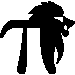
\includegraphics[width=0.075\textwidth]{../Logo}}

\usetheme{Rochester}
\usecolortheme{whale}
%\beamertemplatenavigationsymbolsempty

\AtBeginSection[] {%
	\begin{frame}
		\frametitle{Table of Contents}
		\tableofcontents[currentsection]
	\end{frame}
}

\newenvironment{compactmath}[1][\normalsize]%
	{\begin{minipage}{\textwidth}\vspace{-0.75\baselineskip}#1\begin{equation*}}
	{\end{equation*}\end{minipage}}

\newenvironment{namedframe}[1]%
	{\begin{frame}\frametitle{#1}\framesubtitle{\secname}}
	{\end{frame}}


\title{Probability}
\author{Vincent Macri}
\date{
\includegraphics{../LicenseLogo}\\\copyright{} Vincent Macri, 2017}

\begin{document}
	\frame{\titlepage}
	\section{Introduction}
	\begin{namedframe}{Probability}
		Probability lets us calculate how likely an event is to occur.
		\pause

		Probability has implications in almost every field.  \pause

		For example, in medicine, probability can tell you the likelihood of an operation being successful.
		\pause

		In engineering, knowing the probabilities of different components failing could help you troubleshoot problems faster.
		\pause

		A lot of games have an element of chance. For example, knowing the probabilities of landing on different spaces in Monopoly will tell you which properties will make the most money.
	\end{namedframe}
	\begin{namedframe}{A quick overview of sets}
		\begin{itemize}[<+->]
			\item Sets are an \alert{unordered} collection of \alert{distinct} elements.
			\item Sets are usually labelled with uppercase letters.
			\item The elements of a set are separated by commas inside of braces. Example: $A = \{1,2,3\}$.
			\item A subset of a set contains only elements of the set it is a subset of. For example, a subset of $A$ is $\{1,2\}$.
			\item The empty set (also called the null set) is the set containing no elements. It is written as $\{\}$ or $\varnothing$. It is a subset of all other sets.
			\item A set with $k$ elements has $2^k$ subsets.
			\item The cardinality of a set $A$, written as $n(A)$ is the number of elements in $A$. For example, $n(A) = 3$.
		\end{itemize}
	\end{namedframe}
	\begin{namedframe}{A quick overview of set operations}
		There are two main set operations we deal with.
		\pause
		\begin{description}[<+->]
			\item[Set Union] $A \cup B$ is the set of all elements in $A$ \alert{or} $B$.
			\item[Set Intersection] $A \cap B$ is the set of all elements in $A$ \alert{and} $B$.
		\end{description}
	\end{namedframe}
	\begin{namedframe}{Probability definitions}
		\begin{description}[<+->]
			\item[Sample space] The set of all possible outcomes for an activity (experiment) is the sample space of the experiment. We will call this set $S$.
			\item[Event] An event is a subset of the sample space. We will call this set $E$.
		\end{description}
	\end{namedframe}
	\section{Basics}
	\begin{namedframe}{Equal probability}
		If every possible outcome of an experiment has the same chance of occurring, then we can easily calculate the probability of an event (subset of the sample space) occurring.

		The probability function, $p(E)$ gives us the probability of an event occurring.
		\[p(E) = \frac{n(E)}{n(S)}\]

		Probability is usually written as a number in the range $[0,1]$.
	\end{namedframe}
	\begin{namedframe}{Example}
		We are going to roll a six-sided die.
		\begin{exampleblock}{What is the sample space?}
			\pause
			\begin{compactmath}
				S = \{1,2,3,4,5,6\}
			\end{compactmath}
		\end{exampleblock}
		\pause
		Let's define two events: we roll a composite number ($C$), or we roll a non-composite number ($N$).
		\[C = \{4,6\} \qquad N = \{1,2,3,5\}\]
		\pause
		Then, the change of rolling a composite number is:
		\[p(C) = \frac{n(C)}{n(S)} = \frac{2}{6} = \frac{1}{3}\]
		\pause
		And the chance of rolling a non-composite number is:
		\pause
		\[p(N) = \frac{n(N)}{n(S)} = \frac{4}{6} = \frac{2}{3}\]
	\end{namedframe}
	\begin{namedframe}{Factorial}
		The factorial operation is the product of all integers from $1$ to $n$.
		\pause
		\begin{block}{Definition}
			\begin{compactmath}[\Large]
				n! = 1 \times 2 \times \dots \times n-1 \times n
			\end{compactmath}

			$0! = 1$, because otherwise you would break a lot of math.

			\scriptsize
			Factorial is only defined for non-negative integers. However, using very advanced mathematics it is possible to calculate it for other values.
		\end{block}
		\pause
		\begin{example}
			\begin{compactmath}[\large]
				5! = 1 \times 2 \times 3 \times 4 \times 5 = 120
			\end{compactmath}
		\end{example}
	\end{namedframe}
	\section{Math Elections}
	\begin{namedframe}{Problem}
		The student body of Mackenzie is voting on their 3 favourite parts of math at the school.

		They have 5 options: calculus, vectors, \textrm{\LaTeX{}}, Moodle, and math club.

		Everyone votes for their favourite part, second favourite part, and third favourite part of math at the school.

		These are three separate votes, taken one after another.
	\end{namedframe}
	\begin{namedframe}{Ordered number of options}
		We reason that:
		\begin{enumerate}[<+(1)->]
			\item There are 5 choices for the first spot.
			\item Whatever wins first cannot place second, so we are left with 4 choices for second place.
			\item Whatever options placed first or second cannot place third, so we are left with 3 options for third place.
		\end{enumerate}
		\pause
		This means there are $5 \times 4 \times 3 = 60$ possible combinations.
		
		We can develop the formula for this with factorials:
		\[5 \times 4 \times 3 = 5 \times 4 \times 3 \times \frac{2!}{2!} = \frac{5 \times 4 \times 3 \times 2!}{2!} = \frac{5!}{2!} = 60\]
	\end{namedframe}
	\begin{namedframe}{Unordered number of options}
		If we are only interested in what people's favourite parts of math at the school are, and not the ordering, we can can instead calculate how many combinations of 3 elements there are, with no regard to the order.
		\begin{columns}[c]
			\pause
			\column{0.55\textwidth}

				Take for example, these 6 outcomes:
				\begin{tabular}{|c|c|c|}
					\hline
					\textbf{First} & \textbf{Second} & \textbf{Third}\\\hline
					Math club & Moodle & \textrm{\LaTeX{}}\\\hline
					Math club & \textrm{\LaTeX{}} & Moodle\\\hline
					Moodle & Math club & \textrm{\LaTeX{}}\\\hline
					Moodle & \textrm{\LaTeX{}} & Math club\\\hline
					\textrm{\LaTeX{}} & Math club & Moodle\\\hline
					\textrm{\LaTeX{}} & Moodle & Math club\\\hline
				\end{tabular}
			\pause
			\column{0.45\textwidth}
				If we do not care about ordering, these 6 options become 1 option.

				This means that there are $\frac{60}{3!} = 10$ options for favourite parts of math at Mackenzie when we ignore the ordering.
		\end{columns}
	\end{namedframe}
	\section{Generalizations}
	\begin{namedframe}{Number of ordered options}
		We can calculate the number of \alert{ordered} subsets of size $k$ from a set of cardinality $n$ with the following formula:
		\[P(n,k) = \frac{n!}{(n-k)!}\]
		\pause
		These ordered sets are called \alert{permutations} of $n$ things taken $k$ at a time.
	\end{namedframe}
	\begin{namedframe}{Number of unordered options}
		We can calculate the number of \alert{unordered} subsets of size $k$ from a set of cardinality $n$ with the following formula:
		\[C(n,k) = \frac{n!}{k!(n-k)!}\]
		These unordered selections are called \alert{combinations} of $n$ things taken $k$ at a time.

		\pause
		This formula is also written as:
		\[\binom{n}{k} = \frac{n!}{k!(n-k)!}\]
		And is read as ``$n$ choose $k$''.
	\end{namedframe}
	\section{Yahtzee}
	\begin{namedframe}{Probability of rolling a Yahtzee}
		\begin{exampleblock}{Problem}
			Yahtzee, a game popular with my senior relatives, involves rolling 5 dice. In this game, you get a Yahtzee, which is worth a lot of points, if you roll 5 of a kind.

			All of the dice have six sides.
		\end{exampleblock}
		\begin{exampleblock}{Question}
			What is the probability of rolling a Yahtzee?
		\end{exampleblock}
	\end{namedframe}
	\begin{namedframe}{Calculations}
		First, we will calculate the number of combinations of dice that can be rolled:
		\pause
		\[6^5 = 7776\]
		We will call the set of possible rolls $R$. The cardinality of $R$ is $7776$.
		\pause

		We know that the set of Yahtzee rolls is:
		\begin{align*}
			Y = \{&(1,1,1,1,1), (2,2,2,2,2), (3,3,3,3,3),\\
			      &(4,4,4,4,4), (5,5,5,5,5), (6,6,6,6,6)\}
		\end{align*}
		\pause
		\[p(Y) = \frac{n(Y)}{n(R)} = \frac{6}{7776} = \frac{1}{1296} \doteq 0.00077 = 0.077\%\]
		$\therefore$ the chance of rolling a Yahtzee is about $0.077\%$.
	\end{namedframe}
	\begin{namedframe}{Rolling quadruples}
		\begin{exampleblock}{Question 2}
			How likely is it to roll four of a kind when rolling 5 dice?
		\end{exampleblock}
		We are looking at the change of rolling \alert{exactly} four of a kind. 5 of a kind does \alert{not} count.
	\end{namedframe}
	\begin{namedframe}{Quadruples solution}
		Let's consider the case of rolling quadruple ones.
		\pause

		The chance this happening is with four dice is:
		\[\left(\frac{1}{6}\right)^4 = \frac{1}{1296}\]
		\pause
		But we have five dice, so we must multiply this by the chance of rolling something other than one, and we must multiply by the number of different ways to arrange 4 ones and 1 other die:
		\[\left(\frac{1}{6}\right)^4 \times \frac{5}{6} \times 5 = \frac{25}{7776}\]
		\pause
		The chance of rolling quadruple ones is the same as rolling quadruple twos, threes, etc.. So:
		\[\left(\frac{1}{6}\right)^4 \times \frac{5}{6} \times 5 \times 6 = \frac{25}{1296} \doteq 0.0193\]
	\end{namedframe}
	\begin{namedframe}{Rolling triples}
		\begin{exampleblock}{Question 3}
			How likely is it to roll three of a kind when rolling 5 dice?
		\end{exampleblock}
		We are looking at the change of rolling \alert{exactly} three of a kind. 4 or 5 of a kind do \alert{not} count. We \alert{will} count a 2 of a kind and a 3 of a kind as a triple.
	\end{namedframe}
	\begin{namedframe}{Triples solution setup}
		This is similar to the last problem, so we will some steps for the sake of brevity.
		\pause

		The main difference is that we don't know how many ways we can order three of a kind with two other numbers. With 4 of a kind, this was trivial. It is not longer trivial with three of a kind.
		\[\left(\frac{1}{6}\right)^3 \times \left(\frac{5}{6}\right)^2 \times c \times 6\]
		This is essentially the same formula we used last time, but replacing the number of combinations with the variable $c$. We must use reasoning to figure out $c$.
	\end{namedframe}
	\begin{namedframe}{Triples solution}
		\[\left(\frac{1}{6}\right)^3 \times \left(\frac{5}{6}\right)^2 \times c \times 6\]
		\pause

		We want the number of combinations of $3$ elements from a set of $5$ elements.
		\pause
		\[c = \binom{5}{3} = 10\]
		\pause
		\[\left(\frac{1}{6}\right)^3 \times \left(\frac{5}{6}\right)^2 \times 10 \times 6 = \frac{125}{648} \doteq 0.193\]
	\end{namedframe}
\end{document}
